%	PACKAGES AND OTHER DOCUMENT CONFIGURATIONS

\documentclass[11pt, a4paper]{article} % 10pt font size (11 and 12 also possible), A4 paper (letterpaper for US letter) and two column layout (remove for one column) Use additional titlepage argument to generate this
%\documentclass[12pt, a4paper,twocolumn,titlepage]{article}

%%%%%%%%%%%%%%%%%%%%%%%%%%%%%%%%%%%%%%%%%
% Wenneker Article
% Structure Specification File
% Version 1.0 (28/2/17)
%
% This file originates from:
% http://www.LaTeXTemplates.com
%
% Authors:
% Frits Wenneker
% Vel (vel@LaTeXTemplates.com)
%
% License:
% CC BY-NC-SA 3.0 (http://creativecommons.org/licenses/by-nc-sa/3.0/)
%
%%%%%%%%%%%%%%%%%%%%%%%%%%%%%%%%%%%%%%%%%

%----------------------------------------------------------------------------------------
%	PACKAGES AND OTHER DOCUMENT CONFIGURATIONS
%----------------------------------------------------------------------------------------

\usepackage[english]{babel} % English language hyphenation

\usepackage{microtype} % Better typography

\usepackage{verbatim} % Allows mulitline commenting

\usepackage{amsmath,amsfonts,amsthm} % Math packages for equations

\usepackage[svgnames]{xcolor} % Enabling colors by their 'svgnames'

\usepackage[hang, small, labelfont=bf, up, textfont=it]{caption} % Custom captions under/above tables and figures

\usepackage{subcaption}

\usepackage{booktabs} % Horizontal rules in tables

\usepackage{lastpage} % Used to determine the number of pages in the document (for "Page X of Total")

\usepackage{graphicx} % Required for adding images

\usepackage{enumitem} % Required for customising lists
\setlist{noitemsep} % Remove spacing between bullet/numbered list elements

\usepackage{sectsty} % Enables custom section titles
\allsectionsfont{\usefont{OT1}{phv}{b}{n}} % Change the font of all section commands (Helvetica)

\usepackage{siunitx}

%----------------------------------------------------------------------------------------
%	MARGINS AND SPACING
%----------------------------------------------------------------------------------------

\usepackage{geometry} % Required for adjusting page dimensions

\geometry{
	top=1cm, % Top margin
	bottom=1.5cm, % Bottom margin
	left=2cm, % Left margin
	right=2cm, % Right margin
	includehead, % Include space for a header
	includefoot, % Include space for a footer
	%showframe, % Uncomment to show how the type block is set on the page
}

\setlength{\columnsep}{7mm} % Column separation width

%----------------------------------------------------------------------------------------
%	FONTS
%----------------------------------------------------------------------------------------

\usepackage[T1]{fontenc} % Output font encoding for international characters
\usepackage[utf8]{inputenc} % Required for inputting international characters

\usepackage{XCharter} % Use the XCharter font

%----------------------------------------------------------------------------------------
%	HEADERS AND FOOTERS
%----------------------------------------------------------------------------------------

\usepackage{fancyhdr} % Needed to define custom headers/footers
\pagestyle{fancy} % Enables the custom headers/footers

\renewcommand{\headrulewidth}{0.0pt} % No header rule
\renewcommand{\footrulewidth}{0.4pt} % Thin footer rule

\renewcommand{\sectionmark}[1]{\markboth{#1}{}} % Removes the section number from the header when \leftmark is used

%\nouppercase\leftmark % Add this to one of the lines below if you want a section title in the header/footer

% Headers
\lhead{} % Left header
\chead{\textit{\thetitle}} % Center header - currently printing the article title
\rhead{} % Right header

% Footers
\lfoot{} % Left footer
\cfoot{} % Center footer
\rfoot{\footnotesize Page \thepage\ of \pageref{LastPage}} % Right footer, "Page 1 of 2"

\fancypagestyle{firstpage}{ % Page style for the first page with the title
	\fancyhf{}
	\renewcommand{\footrulewidth}{0pt} % Suppress footer rule
}

%----------------------------------------------------------------------------------------
%	TITLE SECTION
%----------------------------------------------------------------------------------------

\newcommand{\authorstyle}[1]{{\large\usefont{OT1}{phv}{b}{n}\color{NavyBlue}#1}} % Authors style (Helvetica)

\newcommand{\institution}[1]{{\footnotesize\usefont{OT1}{phv}{m}{sl}\color{Black}#1}} % Institutions style (Helvetica)

\usepackage{titling} % Allows custom title configuration

\newcommand{\HorRule}{\color{SteelBlue}\rule{\linewidth}{1pt}} % Defines the gold horizontal rule around the title

\pretitle{
	\vspace{-30pt} % Move the entire title section up
	\HorRule\vspace{10pt} % Horizontal rule before the title
	\fontsize{32}{36}\usefont{OT1}{phv}{b}{n}\selectfont % Helvetica
	\color{Navy} % Text colour for the title and author(s)
}

\posttitle{\par\vskip 15pt} % Whitespace under the title

\preauthor{} % Anything that will appear before \author is printed

\postauthor{ % Anything that will appear after \author is printed
	\vspace{10pt} % Space before the rule
	\par\HorRule % Horizontal rule after the title
	\vspace{20pt} % Space after the title section
}

%----------------------------------------------------------------------------------------
%	ABSTRACT
%----------------------------------------------------------------------------------------

\usepackage{lettrine} % Package to accentuate the first letter of the text (lettrine)
\usepackage{fix-cm}	% Fixes the height of the lettrine

\newcommand{\initial}[1]{ % Defines the command and style for the lettrine
	\lettrine[lines=3,findent=4pt,nindent=0pt]{% Lettrine takes up 3 lines, the text to the right of it is indented 4pt and further indenting of lines 2+ is stopped
		\color{NavyBlue}% Lettrine colour gold DarkGoldenRod
		{#1}% The letter
	}{}%
}

\usepackage{xstring} % Required for string manipulation

\newcommand{\lettrineabstract}[1]{
	\StrLeft{#1}{1}[\firstletter] % Capture the first letter of the abstract for the lettrine
	\initial{\firstletter}\textbf{\StrGobbleLeft{#1}{1}} % Print the abstract with the first letter as a lettrine and the rest in bold
}

%	BIBLIOGRAPHY

\usepackage[backend=biber,style=phys,natbib=true,doi=false]{biblatex} 
%Can equally use numeric citation style without extra phys packaging (but doesn't change capitalisation), or authoryear for alphabetical listing without the codes (resembles APA)

%\addbibresource{references.bib} % The filename of the bibliography

\usepackage[autostyle=true]{csquotes} % Required to generate language-dependent quotes in the bibliography

%    APPENDICES

\usepackage[title]{appendix} %in appendix


 % Specifies the document structure and loads requires packages
\graphicspath{{"/Users/kit gallagher/Documents/Research Review/Report/Figures"}}
\newcommand*{\subscript}[1]{\ensuremath{_\textrm{{\scriptsize #1}}}}

%	ARTICLE INFORMATION

\title{Simulating Liquid Crystals}

%\author{
	%\authorstyle{Christopher Gallagher}}
\author{\authorstyle{Kit Gallagher} 
	%\institution{University of Cambridge \\
	\institution{Supervisors: Prof Erika Eiser, Mr Jiaming Yu}}
% Example of a one line author/institution relationship
%\author{\newauthor{John Marston} \newinstitution{Universidad Nacional Autónoma de México, Mexico City, Mexico}}

\date{\today} % Add a date here if you would like one to appear underneath the title block, use \today for the current date, leave empty for no date
\usepackage[english]{babel}
\usepackage{tabularx}
%\renewcommand{\thefootnote}{\roman{footnote}}  %use roman lettering for footnotes instead
%\usepackage[backend=biber,doi=false]{biblatex}
\addbibresource{reportreferences.bib}
%\AtBeginBibliography{\small}
%----------------------------------------------------------------------------------------
\begin{document}
	
%Your project should contain the following statement on the first page of the project: Except where specific reference is made to the work of others, this work is original and has not been already submitted either wholly or in part to satisfy any degree requirement at this or any other university.	A link to your on-line notebook should also be added to the first page of your report before uploading the project.

\maketitle % Print the title

\thispagestyle{firstpage} % Apply the page style for the first page (no headers and footers)

%	ABSTRACT

\lettrineabstract{The specificity of DNA base-pair interactions gives considerable functional control in the design of anisotropic nano-particles, enabling the formation of liquid crystal phases. This project aims to study the liquid phase behaviour of such non-conventional liquid crystal molecules, with a particular focus on the novel `nunchuck' structure - two rigid rods connected via a flexible linker. The Eiser Group have previously considered intra-molecular interaction potentials at the single-nucleotide level for a single DNA nanoparticle, and I am now implementing these potentials in larger, more coarse-grained models of multiple nanoparticles, through open-source software LAMMPS (Large-scale Atomic/Molecular Massively Parallel Simulator). Such systems are expected to form smectic (layered) phases at high volume fractions. THIS WILL BE EDITED AT THE END}

\section{Introduction}
What are we studying? (brief) - introduce nunchuck particles (but not implementation)
Why are we interested? Applications of this!
% intro to entropically driven transitions

Outline of report

\section{Background}
\subsection{Liquid Crystals}
Include known phases etc - de gennes textbook gives useful milestone references 
\subsection{Onsager Theory}
Introduce theoretical predictions to be validated later
Mathematical derivations may be provided in appendicies
\subsection{Order Parameter}
%smectic order given by frenkel https://pubs.acs.org/doi/pdf/10.1021/j100322a042
%can also use https://www.tandfonline.com/doi/full/10.1080/00268976.2018.1471231

The degree of order in a liquid crystal phase is characterised by an order parameter, chosen such that it is non zero in the ordered phase but vanishes in the isotropic phase. A familiar example of this is the magnetisation $\textbf{M}$ of a ferromagnet; when raised above a critical temperature, the magnetisation vanishes as the ferromagnet undergoes a phase transition. While the choice of order parameter for the nematic phase transition is less intuitive than this, it relies on the formation of genuine long-range orientational order. We may therefore define the angle ($\theta$) between each molecule's axis and the system director, and traditionally let the order parameter S be given by:

\begin{equation}
S_{n} = \left\langle P_{2}(\cos(\theta)) \right\rangle = \left\langle \frac{3}{2}\cos^{2}(\theta) - \frac{1}{2} \right\rangle 
\end{equation}

where $P_{2}$ simply denotes the second Legendre polynomial \cite{deGennes1993}. While $\langle \cos^{2}(\theta) \rangle$ would function alone as the order parameter, this has the useful property of giving unity for a perfectly aligned system, and zero for a completely random system. Further motivation for this choice is provided in Appendix \ref{sec:OrderParamTheory}.

%add description of pair-wise orientational order coeff

Similarly we will find it helpful to define a smectic order parameter $S_{s}$, to characterise the formation of one-dimensional long-range positional order. Intuitively, we expect a non-zero Fourier component of the normalised density along the director \cite{Polson1997}, and so we may write:

\begin{equation}
S_{s} = \frac{1}{N} \left\lvert \sum_{j=1}^{N} \exp \left( {\frac{2\pi}{L}i\textbf{r}_{j} \cdot \boldsymbol{\hat{n}}} \right) \right\rvert
\end{equation}

for a layers of periodicity $L$ perpendicular to the nematic director $\boldsymbol{\hat{n}}$, and where $\textbf{r}_{j}$ denotes the centre of mass position of the $j$th molecule \cite{Dussi2018}.

\subsection{Previous Computational Work} \label{sec:PrevWork}

\section{Methods}
As introduced in Section \ref{sec:PrevWork}, all molecular dynamics simulations were completed in LAMMPS. LAMMPS (Large-scale Atomic/Molecular Massively Parallel Simulator) is a medium coarse-grained, classical molecular dynamics code developed to replicate  solid-state materials and soft matter mesoscopic systems \cite{Plimpton1995, LAMMPS}.


%Can expand on this if needs be, from rapaport

\subsection{Simulation Molecules}
As introduced in Section \textbf{X}, we are considering `nunchuck' molecules formed of two rigid rods connected by a flexible linker, as depicted in Figure \ref{fig:nunchuck_analogy}. However, as the interaction potential of an anisotropic particle is rather complex, it is computationally simpler to consider each molecule as a system of connected spheres, each with a separate isotropic interaction potential (detailed further in Section \ref{pair_potential}).

This is visualised in Figure \ref{fig:nunchuck_implementation}, for rigid rods of aspect ratio 7. The ss-DNA is represented by a further sphere in the centre of the molecule, coloured differently in red to highlight its differing mechanical properties. It has a modified bond angle, so the molecule is bent around this element, and reduced bond rigidity so the particle may also stretch about this point. 

\begin{figure}[ht]
	\hfill  %NOT SURE ABOUT THIS!
	\begin{subfigure}{.4\textwidth}
		\centering
		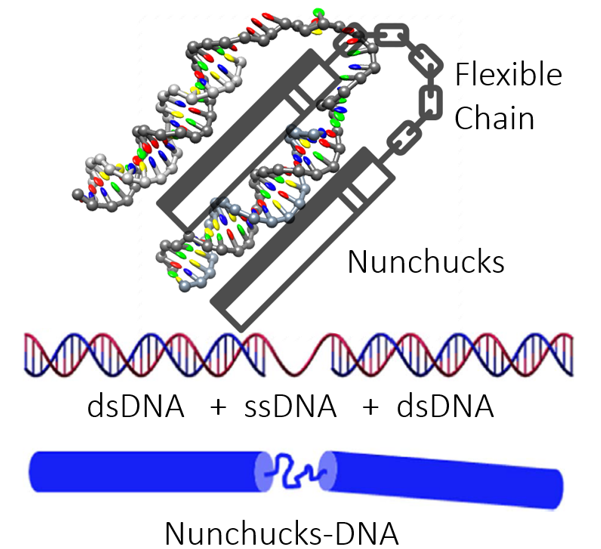
\includegraphics[width=\linewidth]{Figures/nunchucks_artist}  
		\caption{Coarse-grained Model}
		\label{fig:nunchuck_analogy}
	\end{subfigure}
	\hfill %% useful if width of each figure is less the .5\textwidth
	\begin{subfigure}{.4\textwidth}
		\centering
		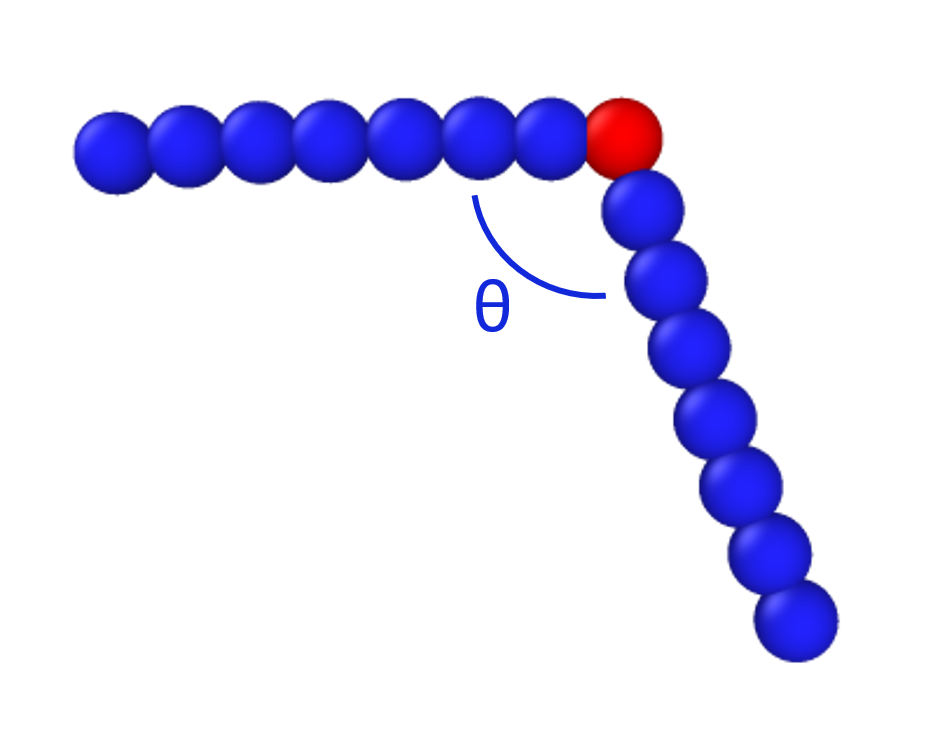
\includegraphics[width=\linewidth]{Figures/nunchuck_profile_coloured}  
		\caption{LAMMPS Implementation}
		\label{fig:nunchuck_implementation}
	\end{subfigure}
	\caption{Depiction analogy between the DNA mesogen and the nunchucks. Note the appearance of the flexible ss-DNA linker between the rigid ds-DNA rods, and the implementation within LAMMPS on the right. The central red sphere, representing the ss-DNA, is given modified bond properties to replicate the nunchuck's flexibility. Figure (a) created by Jiaming Yu (Eiser Group, Cambridge).}
	\label{fig:nunchucks_visual}
	\hfill
\end{figure}

A system of natural units was used in simulations, and replicated in tour results here. Based on the Lennard-Jones potential, the cut-off length and characteristic energy are both set to unity. The simulation timescale is then fixed by the choice of these values, and the mass of the simulation body. 

The physical values for a system may be considered for a specific system (in this case strands of ds-DNA) through scaling via the relevant mass, length scale and energy scale of this system. However the dimensionless simulations presented here may be generalised to any similarly-shaped mesogens; we would expect other systems to display the same behaviour over an appropriate timescale determined by their material properties \cite{Rapaport2004}.

For the nunchuck particles considered, a length scale of \SI{2}{\nano\metre} is used (corresponding to the width of ds-DNA, and hence the diameter of a simulation sphere) \cite{Arnott1972}. It is worth noting that the persistence length of DNA is around \SI{50}{\nano\metre} \cite{Garcia2007}, so the approximation of perfect rigidity is valid for all rods considered here (maximum length \SI{30}{\nano\metre}). Using the standard value of \SI{0.33}{\nano\metre} \cite{Langridge1960} for the average length of a base pair, each sphere corresponds to a sequence of six base pairs. This gives the mass of each sphere as \SI{6.5e-24}{\kilogram}, based on an average formula mass per base pair of \SI{650}{\dalton} \cite{Duewer2018}). 

We may also define the characteristic energy scale; this is formally the depth of the potential well in the full Lennard-Jones potential, but the thermal energy serves as a common approximation \cite{Pan2010} in agreement with experimental data \cite{Wang2002}. Using these values, we find that the characteristic timescale for this system is \SI{79}{\pico\second}. In this context, the simulation timestep would be \SI{0.4}{\pico\second}, and typical simulation of \num{20e6} steps had a total duration of \SI{7.9}{\micro\second}. For \num{1000} particles, this took approximately $8$ hours to run on a standard laptop CPU. %check these



\subsection{Simulation Structure} %was? is? check your tense here!
All simulations in this report were conducted a system of 1000 particles, with a time step of $0.005\tau$, (where $\tau$ is the characteristic time), unless otherwise stated. The system was initially configured in a dilute, isotropic state; a non-trivial process for large numbers of mesogens as molecules must be placed randomly without overlap, to prevent any initial order affecting the formation of ordered phases. I am grateful to Iria Pantazi for writing a python script to automate this process for dilute rigid rod systems, and a generalised version of this is available in the supplementary material. Alternatively, simulations were also initiated from a perfectly ordered square crystalline phase, with all molecules aligned along a common axis. The choice of this axis is arbitrary, as the system is invariant under global rotation \cite{Nos1983}, but is taken to be directed along the y-axis for clarity. Care was taken to ensure molecules did not overlap, and the system was stable in this ordered phase.
%MAYBE INCLUDE CODE IN SUPP MATERIAL?? THINK ABOUT THIS!

All simulations are conducted within an oblong box defined by the Cartesian axes, with periodic boundary conditions used to eliminate surface effects and replicate conditions in the bulk phase \cite{Frenkel2002}. The aspect ratio of this box may be varied, to support phase formation in anisotropic systems, as discussed in Section \textbf{X}. An isenthalpic ensemble was used (where pressure is fixed) to vary the size of the simulation region, allowing sampling of different volume fractions from the same initial configuration. The  microcanonical ensemble, where both the system volume and energy are conserved, was then used to allow the system to reach thermodynamic equilibrium. Time integration was evaluated using the Nose-Hoover thermostat \cite{Nos1984, Hoover1985} natively implemented in LAMMPS \cite{Shinoda2004}.

A typical simulation consists of multiple stages, alternating between these two ensembles to sample the system properties at a range of volume fractions. Approximately \num{2e4} steps are simulated when varying the simulation volume (depending on the resolution of volume fraction sampling), followed by \num{2e6} to allow the system to reach equilibrium in each stage. The output of thermodynamic variables, as well as particle positions, at the end of each stage allows for subsequent calculation of the order parameter at equilibrium. This data was also retrieved at regular intervals during each simulation stage, to track the time evolution of the system.

To ensure stability of the system, a Langevin thermostat \cite{Schneider1978} was also used throughout, and energy conservation was verified over a range of timescales. The damping for all thermostats is equal to the characteristic timescale of the simulation (i.e. unity in natural units).



\subsection{Intermolecular Potential} \label{pair_potential}
A shifted, cut-off Lennard-Jones potential was chosen to represent pair-wise interactions between molecules. While the Lennard-Jones potential \cite{Jones1924a, Jones1924b} has long been the natural choice for molecular dynamics simulations \cite{Stephan2019}, its infinite range introduces computational complexity as interactions between all pairs of particles must be considered. It is therefore increasingly common to use a cut-off version, whereby the potential is set to zero beyond a `cut-off' radius, and here we chose to neglect the entire attractive tail. As well as simplifying the calculations required, this also allows our results to be generalised to any mesogens without attractive inter-molecular forces (that typically favour ordered-phase formation), as any phase transitions observed here must be purely entropically driven. This is commonly known as a soft-core model, where particle overlap is suppressed via this repulsive potential rather than any excluded volume interactions, and is computationally much less demanding \cite{Paolini1993, Hughes2008}.
%can cite frenkel on entropically drive transitions if req

However, this cut-off may cause unphysical behaviour if the potential does not tend to zero smoothly at this point. This is remedied by the addition of a constant term, described in the full form of the pair-wise potential $U_{ij}$ in (\ref{lj_cut}):

\begin{equation} \label{lj_cut}
U_{ij} = 4\epsilon \left[ \left( \frac{\sigma}{r_{ij}} \right) ^{12} - \left( \frac{\sigma}{r_{ij}} \right) ^{6}	\right] + \epsilon \qquad	 r_{ij} < r_{c} = 2^{1/6} \sigma
\end{equation}

Here $\sigma$ and $\epsilon$ are the relevant length and energy scales of the system, formally corresponding to the particle separation at which the $U_{ij} = 0$, and the depth of the potential well. It is worth noting that the effects of this truncation and shift on the overall thermodynamic quantities are well documented \cite{Stephan2020, Shaul2010}, and changes in lyotropic properties are negligible in 3D bulk liquids with a conserved particle number \cite{Smit1991}. 


 
\subsection{Analysis}

The visualisation freeware Ovito \cite{Ovito} has been employed to animate the molecule motion over the simulation period, and was used to generate all molecular images presented here. Thermodynamic variables, such as internal energy and pressure, were extracted to track the system's progress towards equilibrium, and verify its stability.

The volume fraction and nematic order parameter were computed for comparison with Onsager's theorem, as detailed in Section \textbf{X}. Calculation of the order parameter is complicated by the absence of an imposed director (ie if no electric field is applied), and we use the approach taken by Eppenga and Frenkel \cite{Eppenga1984} which is reproduced in Appendix \ref{sec:OrderParamCalc}. %or dussi 2018 or many others

Further analysis included the calculation of the smectic order parameter, and pair-wise orientational correlation coefficient, detailed in Section \textbf{X}. All scripts for data extraction and analysis were written by the author, \textit{and can be found in the supplementary material?}.



\section{Rigid Rod Simulations}
Used to benchmark sys etc and demonstrate techniques to identify phase transitions.
Detail nematic phase transition (longrun4) and validation through onsager theory
Extend this with the longer rods which continue to confirm this theory

Initially, a system of rigid rods was used to verify the analysis methods applied in this report, in comparison with the predictions made by Onsager's theory in Section \textbf{X}. We focus specifically on the phase transition between the isotropic and nematic phased, as this system is well studied, and these predictions have been separately verified computationally through both Monte Carlo and molecular dynamics simulations \textbf{cite}, (\textit{and experimentally?}).

For rigid rods with an aspect ratio of 10, we expect this lyotropic phase transition to occur at a volume fraction of $\phi  = 0.4$, according to \textbf{ref equation}. We consider a system of 1000 rigid rods, formed of 10 sequentially connected `balls' (force-centres), and apply alternating stages of contraction (where the volume fraction is increased) and equilibration (where the volume is held constant). Each contraction stage consists of between \num{1e4} and \num{5e4} steps (chosen to identify the critical volume fraction with maximal resolution, while verifying the order parameter is approximately constant outside of this), while the equilibration stage runs for \num{2e6} steps. In this way we are able to confine the possible critical volume fraction to the range $0.39 < \phi< 0.44$, as observed in Figure \ref{fig:rr_nemorderparam}, in good agreement with Onsager's prediction of $\phi = 0.4$.

\begin{figure} [h!]
	\centering
	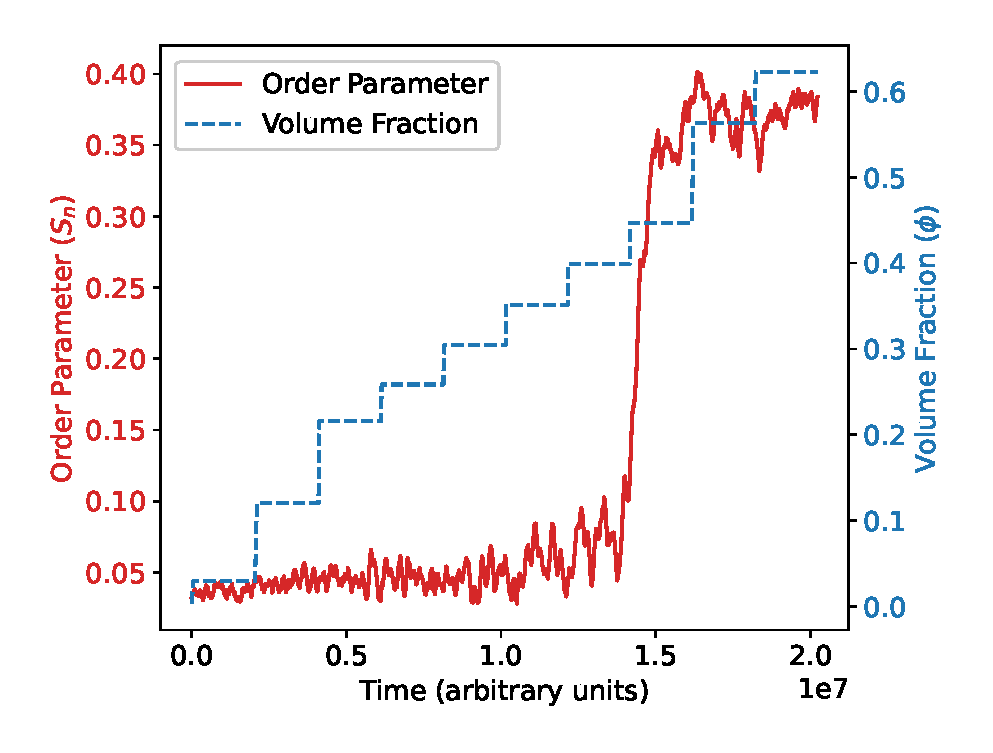
\includegraphics[width=0.7\linewidth]{Figures/rigidrod_nemorderparam}
	\caption{The evolution of the volume fraction ($\phi$) and the nematic order parameter ($S_{n}$) over the timescale of the simulation, for a system of 1000 rigid rods with aspect ratio 10. The phase transition is observed through a discrete change in the order parameter (in red), occurring after the volume fraction is increased above $0.4$. Note that the contraction steps (where volume fraction is changed) are not of equal durations, and so do not correspond to equal changes in the system volume; rather they are chosen to highlight the phase transition. The timescale of contraction is much less that the timescale of equilibration, but the changes in volume fraction are not instantaneous, despite their appearance here.}
	\label{fig:rr_nemorderparam}
\end{figure}
%maybe tidy up figure; add symbols to axes labels and plot volume fraction with a dashed line (with legend) to make clearer for colour-blind. also remove title formally (and tight layout?)


\subsection{Crystalline Configuration}
Explain motivation for running simulation in reverse
Validate location of nematic phase transition
Introduce additional smectic phase transition (is there literature on the predicted volume fraction here?)
This last point may be supported by recent plots fortuitously gained when looking into diffusion.
explain uncertainty on nature of nematic-> smectic transition

\section{Nunchuck Simulations}
Explain two approaches taken here; fixed angle and fixed rigidity
describe the challenges in phase identification here, with references if possible


describe quasi-nematic phase seen in both cases
include picture of herringbone-like structure with fixed angle
include angle distribution for fixed rigidity

\subsection{Orientational Order Parameter}
introduce new method to characterise this
detail spherical harmonics approach to calculation in the appendix?

Describe alternative approaches
LOOK INTO BIAXIAL PHASE FURTHER

\section{Dynamic Properties}
Explanation this has only been considered recently, and is much less well understood, as much of the prior simulation work was using MC simulations, which can only predict static properties.
Simplest dynamic property is diffusive coefficient.

Mention simulation complications with periodic bc, and how this was accounted for?
Give power law prediction and my verification of this in dilute systems.
include plots of diffusion coefficient over vol frac for full transition, and rms displacement boxes

Go on to david's theories for dilute and semi-dilute systems? \textit{also review onsager definitions here?}

Explain role in verification of phase formation, particularly for the smectic phase aligned along the y axis.
\section{Conclusion}
Summarise key results from above, and emphasise their importance 
Also give limitations of results obtained, and suggest direction for further work (for each section?)

\section*{Acknowledgements}
I wish to thank my project supervisor (Prof Erika Eiser), and my day-to-day supervisor (Mr Jiaming Yu), as I am very grateful for their continual teaching and advice, and for the initial code provided by Jiaming Yu to run single-stage, rigid-rod simulations. I am also indebted to Prof Daan Frenkel for the kind insights he offered.

%\clearpage
\printbibliography

\begin{appendices}

\section{Onsager Theory}
\section{Nematic Order Parameter} 
\subsection{Theoretical Outline}\label{sec:OrderParamTheory}
Here I endeavour to outline the motivation for the nematic order parameter used throughout this report, based on the work of Eppenga and Frenkel \cite{Eppenga1984, Frenkel1982}. The nematic phase may be differentiated from the isotropic phase by the formation of cylindrical symmetry, as opposed to the spherical symmetry of the isotropic phase. The deviation from spherical symmetry may be quantified through a set of order parameters $f(\theta, \phi)$ \cite{Zannoni1979}. when considering the axially symmetric nematic phase, independent of $\phi$, $f(\theta, \phi)$ may be generally expressed in the basis of all even Legendre polynomials $P_{2l}$:

\begin{equation}
f(\theta) = \sum_{l=0}^{\infty} a_{2l} P_{2l}(\cos(\theta))
\end{equation}

where $\theta$ is the angle between the molecular orientation and the axis of symmetry of the system. Note that odd-ordered terms are neglected for nonpolar molecules, as the director may point in either of two antiparallel directions and so all odd Legendre polynomials average to zero \cite{Parsons1979}.

In an isotropic phase, $a_{2l}$ vanishes for all $l>0$, so all angular dependence vanishes. More generally,  quantities $\langle P_{2l}(\cos(\theta)) \rangle$ may be used at the order parameter of the system, with the second order term being referred to as the nematic order parameter. Averaging over a population of $N$ molecules, we can therefore write the nematic order parameter $S_{n}$ as:

\begin{equation}
S_{n} = \frac{1}{N} \left\langle \sum_{i=1}^{N} \left( \frac{3}{2} \cos^{2}(\theta_{i})-\frac{1}{2} \right) \right\rangle
\end{equation}

\subsection{Calculation}\label{sec:OrderParamCalc}
The method given above in Appendix \ref{sec:OrderParamTheory} relies on knowledge of the system-wide nematic director (ie the axis of symmetry of the cylindrical phase), to define $\theta_{i}$. However, this is not always possible in physical systems where such a unique direction is not externally imposed.

Instead, as detailed by Frenkel et al. \cite{Frenkel1985}, we maximise the expression:

\begin{equation}
S^{\prime}_{n}(\boldsymbol{\hat{n}^{\prime}}) = \frac{1}{N} \left[ \sum_{i=1}^{N} \left( \frac{3}{2} (\boldsymbol{\hat{n}^{\prime}} \cdot \boldsymbol{\hat{u}_{i}})^{2}-\frac{1}{2} \right) \right]
\end{equation}

where $\hat{u_{i}}$ denotes the orientation of the individual molecular axes in the laboratory frame. This may be written further as:

\begin{equation}
S^{\prime}_{n} = \frac{1}{N} \left\langle \boldsymbol{\hat{n}^{\prime}} \cdot \textbf{Q} \cdot \boldsymbol{\hat{n}^{\prime}}  \right\rangle, \qquad where \enspace \textbf{Q}_{i} = \frac{3}{2} \boldsymbol{\hat{u}_{i}}\boldsymbol{\hat{u}_{i}}-\frac{1}{2}\textbf{I}
\end{equation}

The tensor order parameter $\langle \textbf{Q} \rangle$ is a traceless symmetric 2nd-rank tensor, with three eigenvalues $\lambda_{+}, \lambda_{0}, \lambda_{-}$ \cite{Eppenga1984}. We typically take the largest eigenvalue $(\lambda_{+})$ as the nematic order parameter, a good approximation in large N limit.
In practice, we actually calculate the eigenvalues of the related tensor $\textbf{M}$:

\begin{equation}
\textbf{M} =  \frac{1}{N} \sum_{i=1}^{N} \boldsymbol{\hat{u}_{i}}\boldsymbol{\hat{u}_{j}}
\end{equation}

as this shares eigenvectors with $\textbf{Q}$, and has eigenvectors $\mu_{n}$ related to $\lambda_{n}$ by: $\mu_{n} = 2/3 \lambda_{n} + 1/3$.

It is worth noting $\lambda_{+}$ is bound above zero, and so does not reach zero in the isotropic phase as would be expected. It is common to use $S =  -2\lambda_{0}$ when considering such disordered systems, as this fluctuates about an average much closer to zero \cite{Mountain1977}. I have not done so in the results presented here, to give continuity in the order parameter over the transition (where the focus on this report lies), however this has meant that the average order parameter in the isotropic phase is slightly above zero.


\section{Code?}

\end{appendices}

\end{document}


%%%%%%%%%%%%%%%%%%%%%%%%%%%%%%%%%%%%%%%%%
% Wenneker Article
% LaTeX Template
% Version 2.0 (28/2/17)
%
% This template was downloaded from:
% http://www.LaTeXTemplates.com
%
% Authors:
% Vel (vel@LaTeXTemplates.com)
% Frits Wenneker
%
% License:
% CC BY-NC-SA 3.0 (http://creativecommons.org/licenses/by-nc-sa/3.0/)
%
%%%%%%%%%%%%%%%%%%%%%%%%%%%%%%%%%%%%%%%%%
